\newpage
\section{Sponza 的纹理模糊与画面闪动}
\begingroup
\setlength{\parindent}{2\ccwd}
\setlength{\parskip}{5pt}
想象蓝色挂毯的斜边正好穿过一个像素。这个像素一部分是蓝布，一部分是后面的石柱，人眼希望看到按覆盖面积混合出来的颜色。一次只在像素中心取样，可能只取到蓝色。让下一帧在同一像素内稍微挪一下，便能补上石柱的颜色。这个办法叫时间抗锯齿（TAA）。它依赖一个简单条件：两次采样都在为同一个显示像素积累观测。如果把旧颜色每帧再往邻居那里挪一次，就会逐渐弄糊原本清楚的边缘。

在 Vulkan 编辑器打开 Sponza 中庭，将镜头对准拱门和挂毯。旧展示场景指定的内部宽度只有 320 像素，场景面板却会随窗口变宽。挂毯的细线在那张小图里已经混成相同的像素，放大显示时便只剩一条模糊的色带。查画质时要同时记录内部输出和面板的实际像素尺寸。缩小整张桌面截图，会让本来明显的差别消失。

下一次实验固定相机、场景和灯光，保持渲染宽高都是 $161\times91$。用 16 个不同的子像素位置循环采样，保存 32 帧的 GPU 读回。所有灯逐盏计算，关掉随机反射和间接光。这样第二轮的亮度变化只可能来自采样位置和 TAA。修改前后 16 个原始输入的 SHA-256 相同，可以比较第 17--32 帧的输出。

\subsection{历史颜色的采样位置}
旧代码把当前表面投回上一帧带偏移的投影。镜头尽管没动，两次采样点也可能相差半个像素。历史颜色已经在上一帧混合过，再从四个相邻像素之间插值一次，会把柱边的一部分颜色摊到旁边。轮廓上，某次射线打中柱子，下一次却打到背景，旧代码有时直接舍弃历史。两件事一起出现，静态画面就既软又闪。

\begin{Code}
// 旧版 TAA.comp 中的两句。previousVP 包含上一帧的采样偏移。
vec4 clip = previousVP * pos;
vec2 oldPixel = toPixel(clip) - .5;
\end{Code}
\loc{Redflag/src/Redflag/Renderer/ScreenSpace/Shaders/TAA.comp}
现在分别保存实际取样用的投影和偏移前的稳定投影。若相机位置、模型和光照都没变，把本次观测累加到同一个显示像素。若相机确实移动，用稳定投影计算它在两帧之间移动了多少，再检查旧像素是否来自相近的表面。切镜头、换场景或改变几何后须清空历史。第一帧完全采用当帧颜色，第二帧最多取一半旧颜色，随后逐步接纳更多历史。

\begin{Code}
// 新版中 previousVP 和 stableVP 都是偏移前的相机矩阵。
vec4 clip = previousVP * pos;
vec2 oldPixel = vec2(p) + toPixel(clip) - toPixel(stableVP * pos);
\end{Code}
\loc{Redflag/src/Redflag/Renderer/ScreenSpace/Shaders/TAA.comp}

\newpage
\subsection{静止镜头的亮度变化}
先从真实数据里只取一个像素。左上角为 $(0,0)$，在 $(98,61)$，旧版本第 17 帧的显示亮度是 0.45782，第 18 帧变成 0.13868，相减为 $-0.31914$。修正后，两帧分别是 0.42912 和 0.41339，相减约为 $-0.01573$。这点选在变化明显的地方，能看清计算过程。整幅图的结论要用上全部像素，包括没有变化的背景。

这里用 0 表示黑、1 表示白。程序给两版输出使用相同的曝光 4 和同一条显示曲线，再把三个颜色分量折成一个代表明暗的数 $Y=0.2126R'+0.7152G'+0.0722B'$。撇号表示已经做过显示转换。这个数用于比较屏幕上的明暗变化，单位是满量程的一份。它和照度计测到的照度不同。

若四个像素分别变化了 $0,0,+0.1,-0.1$，直接取平均会得到零，把一亮一暗抵消了。先平方，就能同时保留变亮和变暗的幅度。再求平均并开平方，数值又回到原来的亮度单位：
\[
 \sqrt{(0^2+0^2+0.1^2+(-0.1)^2)/4}=\sqrt{0.005}\approx0.07071.
\]
每个像素有 16 个不同的取样位置。测试先完整画一轮，让 TAA 存下能供下一轮使用的颜色，再开始计量。第二轮的 16 张图可以两两相邻配出 15 对，每张有 $161\times91=14\,651$ 个像素，共得到 $219\,765$ 个亮度差。对这些差值执行上面的计算，旧版得到 0.06584257，修正版得到 0.00553348。换成 0--255 的显示刻度，两项均方根约为 16.79 和 1.41 个灰阶。单个像素的变化仍可能更大。

\begin{Code}
# 按 tests/temporal_quality.py / measure 简写
change = lum[1:] - lum[:-1]  # 同一像素在相邻两帧的亮度差
rms_change = rms(change)     # 所有像素的差值平方，求平均，再开方
\end{Code}
测试的失败门槛是另行选择的数。0.01 相当于满量程的 1\%，约 2.55 个灰阶，高于本次修正后的 1.41、低于旧版的 16.79，给相同场景的微小波动留出余量。边缘误差门槛 0.005 同样来自本案例的新旧测量。两道门槛是本项目针对这个固定镜头的工程约定；改变曝光、相机或参考样本后，要先重新建立基线才适合比较。

\newpage
\begin{center}
\begin{minipage}{.48\linewidth}\centering
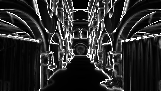
\includegraphics[width=\linewidth]{../../../output/validation/temporal/before-motion.png}\\原来的 TAA\end{minipage}\hfill
\begin{minipage}{.48\linewidth}\centering

\includegraphics[width=\linewidth]{../../../output/validation/temporal/after-motion.png}\\稳定投影修正后\end{minipage}
\end{center}
两张图都把连续帧的亮度变化放大 8 倍。越亮的地方闪动越明显；相机始终静止。这是 GPU 输出的差值图，原始像素保存在测量目录，读者可以独立重算。

\noindent\begin{tabularx}{\linewidth}{@{}Xrr@{}}\toprule
同一静止镜头，第 17--32 帧 & 修改前 & 修改后\\\midrule
相邻帧亮度差的均方根 & 0.06584 & 0.00553\\
与 16 次采样均值的边缘梯度误差（均方根） & 0.03672 & 0.00170\\
与同一参考的线性 RGB 均方误差 & 0.0008634 & 0.0000120\\\bottomrule
\end{tabularx}

第一行回答“同一处是否还在跳”。第二行先把 16 帧输出取平均，再比较相邻像素的亮度差和参考图是否一致，能发现一张稳定但细节被磨平的图。第三行在曝光前比较颜色。两种均方根都使用固定显示变换，亮度范围是 0 至 1。这里的参考是指定采样位置的均值，测的是时间合成误差。

另用编辑器实际场景里的三盏点光源和带纹理模型，在 $320\times180$ 固定镜头下单独测试探针噪声。逐灯求和的直接光逐帧相同。对第 9--24 帧，DDGI 每探针方向发两条光线时，平均 3.89\% 的像素有至少一个通道在相邻帧变化超过三个 8 位灰阶；增至十六条后为 1.03\%。这组数据测的是间接光自己的变化。调高探针样本数和修正 TAA 的作用可以分别检查。

在仓库根目录运行 \path{tests/run_screen_effects.cmd}。测试同时覆盖挂毯纹理方向、四个 UV 采样点、相机横移后仍有效的历史以及重置后的第一帧。本机使用原始输入时，静止帧亮度差超过 0.01 或边缘误差超过 0.005，脚本就报告失败。换显卡导致输入哈希变化时会标明条件，并使用本次生成的参考图核对 TAA。逐帧原图用于追查误差位置，单次 RenderDoc 捕获用于核对着色器实际读了哪两帧。

\loc{tests/temporal_quality.py}
\loc{output/validation/temporal/metrics.json}

\newpage
\subsection{挂毯上的细纹}
两次窗口捕获使用同一相机和布光。从灯旁挂毯的金色花纹向上看，低分辨率输出把相邻细线混在一起。改用面板原始尺寸后，更细的纹样和拱门上的砖缝仍然可分辨。编辑器的分辨率选项 \texttt{Native} 会跟随面板实际像素；需要低成本预览时也可手动选小图。下面使用同一版本切换分辨率，单独显示尺寸带来的差别。

\begin{center}
\begin{minipage}{.48\linewidth}\centering
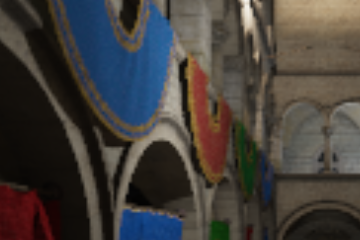
\includegraphics[width=\linewidth]{../../../output/validation/temporal/editor-detail-320.png}\\输出 $320\times207$，面板 $948\times613$\end{minipage}\hfill
\begin{minipage}{.48\linewidth}\centering
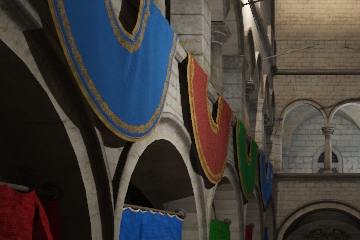
\includegraphics[width=\linewidth]{../../../output/validation/temporal/editor-detail-native.png}\\输出与面板同为 $948\times613$\end{minipage}
\end{center}
上图从实际窗口截取相同大小的 $360\times240$ 局部，完整截图保存在 \path{output/rhi/}。两幅画面的取样设置相同。

贴近挂毯后，清晰度还受贴图自身限制。当前光追预览将底色图的最长边限制为 512，按 UV 做双线性读取。后续比较更高分辨率贴图和按像素覆盖范围选层的过滤时，可以继续用同一块金边做静止近景，再缓慢后退检查细线闪动，分别记录显存和帧差。

\subsection{四色贴图与模型根节点}
第一次用编辑器相机检查 Sponza 的光追视图，只能看到一大片地面。读取追踪用的包围盒发现，模型沿 $x$ 方向仍从约 $-1921$ 延伸到 $1800$。导入文件的根节点带有 0.008 的缩放。光栅绘制逐个访问节点、继承了这个缩放；单独的追踪加载路径用了预变换网格，得到的尺寸不同。现在编辑器的两个渲染入口共用 \texttt{VisitModelMeshes}，从同一个根节点开始累积变换，逐子网格应用实体指定的材质。

另一个假象是贴图消失后仍能看到材质颜色。测试用一张四格图检查这一点，上排红、绿，下排蓝、白。模型的根缩放为 0.5，实体另指定颜色倍率 $(0.5,0.25,1)$。修复过程中左上格曾读出 $(0.5,0.25,1)$，说明只剩实体底色。检查项目内的 Assimp 发现，glTF 导入器把内嵌图像写作 \texttt{*0}，当前版本按文件名查询的接口找不到这个编号。现在先解析编号、读取模型自带的图像，再按三角形重心坐标插值 UV，最后查底色。左上格现在是 $(0.5,0,0)$，另外三格也分别通过 GPU 读回。这样既能查到丢图，又能辨别上下翻转和错误缩放。
\loc{tests/fixtures/TextureQuad.gltf}
\endgroup
